%----------------------------------------------------------------------------------------
%	PACKAGES AND OTHER DOCUMENT CONFIGURATIONS
%----------------------------------------------------------------------------------------

\documentclass[11pt]{scrartcl} % Font size

%%%%%%%%%%%%%%%%%%%%%%%%%%%%%%%%%%%%%%%%%
% Wenneker Assignment
% Structure Specification File
% Version 2.0 (12/1/2019)
%
% This template originates from:
% http://www.LaTeXTemplates.com
%
% Authors:
% Vel (vel@LaTeXTemplates.com)
% Frits Wenneker
%
% License:
% CC BY-NC-SA 3.0 (http://creativecommons.org/licenses/by-nc-sa/3.0/)
% 
%%%%%%%%%%%%%%%%%%%%%%%%%%%%%%%%%%%%%%%%%

%----------------------------------------------------------------------------------------
%	PACKAGES AND OTHER DOCUMENT CONFIGURATIONS
%----------------------------------------------------------------------------------------

\usepackage{amsmath, amsfonts, amsthm} % Math packages

\usepackage{listings} % Code listings, with syntax highlighting

\usepackage[english]{babel} % English language hyphenation

\usepackage{graphicx} % Required for inserting images
\graphicspath{{Figures/}{./}} % Specifies where to look for included images (trailing slash required)

\usepackage{booktabs} % Required for better horizontal rules in tables

\numberwithin{equation}{section} % Number equations within sections (i.e. 1.1, 1.2, 2.1, 2.2 instead of 1, 2, 3, 4)
\numberwithin{figure}{section} % Number figures within sections (i.e. 1.1, 1.2, 2.1, 2.2 instead of 1, 2, 3, 4)
\numberwithin{table}{section} % Number tables within sections (i.e. 1.1, 1.2, 2.1, 2.2 instead of 1, 2, 3, 4)

\setlength\parindent{0pt} % Removes all indentation from paragraphs

\usepackage{enumitem} % Required for list customisation
\setlist{noitemsep} % No spacing between list items

%----------------------------------------------------------------------------------------
%	DOCUMENT MARGINS
%----------------------------------------------------------------------------------------

\usepackage{geometry} % Required for adjusting page dimensions and margins

\geometry{
	paper=a4paper, % Paper size, change to letterpaper for US letter size
	top=2.5cm, % Top margin
	bottom=3cm, % Bottom margin
	left=3cm, % Left margin
	right=3cm, % Right margin
	headheight=0.75cm, % Header height
	footskip=1.5cm, % Space from the bottom margin to the baseline of the footer
	headsep=0.75cm, % Space from the top margin to the baseline of the header
	%showframe, % Uncomment to show how the type block is set on the page
}

%----------------------------------------------------------------------------------------
%	FONTS
%----------------------------------------------------------------------------------------

\usepackage[utf8]{inputenc} % Required for inputting international characters
\usepackage[T1]{fontenc} % Use 8-bit encoding

\usepackage{fourier} % Use the Adobe Utopia font for the document

%----------------------------------------------------------------------------------------
%	SECTION TITLES
%----------------------------------------------------------------------------------------

\usepackage{sectsty} % Allows customising section commands

\sectionfont{\vspace{6pt}\centering\normalfont\scshape} % \section{} styling
\subsectionfont{\normalfont\bfseries} % \subsection{} styling
\subsubsectionfont{\normalfont\itshape} % \subsubsection{} styling
\paragraphfont{\normalfont\scshape} % \paragraph{} styling

%----------------------------------------------------------------------------------------
%	HEADERS AND FOOTERS
%----------------------------------------------------------------------------------------

\usepackage{scrlayer-scrpage} % Required for customising headers and footers

\ohead*{} % Right header
\ihead*{} % Left header
\chead*{} % Centre header

\ofoot*{} % Right footer
\ifoot*{} % Left footer
\cfoot*{\pagemark} % Centre footer

%----------------------------------------------------------------------------------------
%	CAZZATE CHE HA AGGIUNTO MARCO
%----------------------------------------------------------------------------------------

\usepackage[linkcolor=cyan,colorlinks=true,linktocpage=true]{hyperref}
\usepackage{tabularray}

\newcommand{\abs}[1]{\left\lvert #1\right\rvert}
\newcommand{\exval}[1]{\left\langle #1 \right\rangle}

%\renewcommand{\thesubsection}{\thesection.\alph{subsection}}
 % Include the file specifying the document structure and custom commands

%----------------------------------------------------------------------------------------
%	TITLE SECTION
%----------------------------------------------------------------------------------------

\title{	
	\normalfont\normalsize
	\textsc{University of Pisa, Physics Department}\\ % Your university, school and/or department name(s)
	\vspace{25pt} % Whitespace
	\rule{\linewidth}{0.5pt}\\ % Thin top horizontal rule
	\vspace{20pt} % Whitespace
	{\huge Simulation of $2$-dimensional Ising model}\\ % The assignment title
	\vspace{12pt} % Whitespace
	\rule{\linewidth}{2pt}\\ % Thick bottom horizontal rule
	\vspace{12pt} % Whitespace
}

\author{\LARGE Marco Cocciaretto,  \LARGE Miriam Patricolo} % Your name

\date{\normalsize\today} % Today's date (\today) or a custom date

\begin{document}

\maketitle

\section*{Abstract}
We ran a simulation of a $2$-dimensional Ising model; our scope was to study the behaviour of the system near its critcal temperature $T_c$ and to derive its critical exponents. Since our computers are not infinitely powerful, we simulated the system for finite lattice sizes, but we were able to study the phase transitions through Finite Size Scaling, which enabled us to understand how the system would behave if it were of infinite size.

\section{Ising model}
The Ising model represents the interaction between classical spins fixed on a grid. Its hamiltonian is:
\begin{equation}
	\label{ising}
	H = -J \sum _{\langle i,j \rangle} S_i S_j - h\sum_i S_i \equiv H\left[\left\{S_i\right\}\right]
\end{equation}
Where $S_i =\pm 1\, \forall i$ and $\langle i,j \rangle$ indicates that the sum must be computed $\forall i,j$ that satisfy the proximity conditions, which in our case means that the sites $i$ and $j$ must be adjacent in our grid, either vertically or horizonatally. The collection $\left\{S_i\right\}$ represents a state of the system, so that we can write the probability distribution of the states:
\begin{equation}
\label{distribution}
\rho\left(\left\{S_i\right\}\right) = \frac{1}{Z} \exp \left(-\beta H\left[\left\{S_i\right\}\right]\right)
\end{equation}
\begin{equation}
Z = \sum_{\left\{S_i\right\}} \exp \left(-\beta H\left[\left\{S_i\right\}\right]\right)
\end{equation}
Where $\beta = 1/(k_B T)$ and $T$ is the temperature of the system. In our simulation, we fixed the following quantities:
\begin{equation}
	\label{choice}
	\begin{array}{c}
		k_B = 1 \\
		J = 1 \\
		h = 0
	\end{array}
\end{equation}
\subsection{Continuous phase transition}
With our choice \eqref{choice}, in the thermodynamical limit, we expect to find a continuous phase transition at an inverse temperature:
\begin{equation}
	\label{bta_theory}
	\beta _c = \frac{1}{T_c} \simeq 0.4406868
\end{equation}
In a neighbourhood of $\beta _c$, we expect a critical behaviour of the system described by the variable $t\equiv (T-T_c)/T_c \propto\beta - \beta _c$ and the power laws:
\begin{eqnarray}
	\label{power}
	\xi \sim \abs{t}^{-\nu} & \\
	\exval{M} \sim \abs{t} ^{\beta} & \quad t<0\\
	\chi \equiv \frac{\partial \exval{M}}{\partial h} = \frac{V}{T}\left(\exval{M^2}-\exval{M} ^2\right)\sim \abs{t} ^{-\gamma} & \\
	C \equiv \frac{\partial \exval{\epsilon}}{\partial T} = \frac{V}{T^2}\left(\exval{\epsilon^2}-\exval{\epsilon} ^2\right) \sim \abs{t}^{-\alpha} &
\end{eqnarray}
Where $\xi$ is the correlation length, $V$ is the volume of the system, $M$ is the magnetization density, $\epsilon$ is the energy density, $\chi$ is the magnetic susceptibility and $C$ is the thermal capacity.
The theoretical values of the critical exponents in a $2$-dimensionsonal Ising model are the following:
\begin{equation}
\label{exponents}
\alpha = 0 \quad \beta = 1/8 \quad \gamma = 7/4 \quad \nu =1
\end{equation}

\section{Metropolis}
\label{metropolis}
In order to sample our system, we devised a Markov chain that we implemented using an \textit{ad hoc} version of the Metropolis algorithm, which can be summarized along these lines:
\begin{enumerate}
	\item Let us call the current state of the system $S$
	\item We select a site of the lattice and we compute a \textit{trial} spin value for that site, i.e. we invert the sign of the spin, so that if we substituted the current value of the spin in that site with the trial value, we would end up in a new state that we call $T$ 
	\item Using \eqref{distribution} we can compute the probabilities for both states, called $p_S$ and $p_T$. If we select the $i$-th site, the ratio of the probabilities is:
	\begin{equation}
		\frac{p_T}{p_S} = \exp\left(-2\beta\left(\sum _{\langle i,j \rangle} S_j\right) S_i\right)
	\end{equation}
	Note that the sum above only has $4$ terms given our proximity conditions, since $i$ is fixed in the sum
	\item Now the Metropolis test is run: the state $T$ becomes the actual state of the system with probability $p_T/p_S$ (if $p_T/p_S > 1$ then the state $T$ always becomes the new state of the system)
	\item We repeat the steps above for all the sites of the system
\end{enumerate}

\section{Bootstrap}
\label{bootstrap}
Markov chains produce data which are not uncorrelated (each state has a well defined probability of being sampled given the previous state), rendering error estimation more bothersome than usual. To account for this, we used the bootstrap block resampling technique. Let us consider an array of data points of size \texttt{measures} and let us assume that this array represents the states of the lattice during the simulation\footnote{The physical quantities that we want to compute can be derived from just 2 arrays, which store the magnetization density and the energy density of the states explored by the Markov chain, so it is not necessary to save each spin configuration during the simulation and the bootstrap algorithm can be implemented using these arrays}, then, if we want to compute the error associated to a given observable, the bootstrap algorithm runs as follows:
\begin{itemize}
	\item Selects a resampling size \texttt{bin{\_}size}
	\item Extracts a random number \texttt{k} in the range of \texttt{measures}
	\item Resamples all the \texttt{bin{\_}size} consecutive elements of the array starting from the \texttt{k}-th element and stores them into another array\footnote{If $\mathtt{k}+\mathtt{bin{\_}size} > \mathtt{measures}-1$, then the algorithm resamples the last \texttt{bin{\_}size} elements of the array}
	\item Repeats the last two steps $\mathtt{measures}/\mathtt{bin{\_}size}$ times, storing the data in the same array as the previous step, so that the resampled array would have approximately the same size (exactly the same size if \texttt{bin{\_}size} is a divisor of \texttt{measures}) of the initial array
	\item Calculates the desired observable from the resampled array, saving it into another array
	\item Repeats the steps above for an arbitrary times, which we called \texttt{resamplings}, so that the array of observable would end up having \texttt{resamplings} elements (we fixed $\mathtt{resamplings}=100$)
	\item Computes the standard deviation of the array of observables and stores its value into another array
	\item Repeats the steps above for increasing values of \texttt{bin{\_}size}. Specifically, the algorithm executes the line $\mathtt{bin{\_}size} = \mathtt{bin{\_}size}*2$ at the end of the last step
	\item Finally, returns the maximum value of the array of standard deviations, which we infer to be the correct estimate of the error of that given observable
\end{itemize}
The central values of the observables are calculated directly from the starting arrays.

\section{Simulation}
Basically, our simulation does the following:
\begin{enumerate}
	\item Reads all the variables needed to run the simulation from \texttt{.txt} files which had been created for this purpose.
	\item Suppose the sides of the lattice are long $L$, then the algorithm creates a square lattice matrix of size \texttt{Nlatt}, so that $L = a\mathtt{Nlatt}$, where $a$ is the distance between two adjacent spins, initializing it in 3 possible states, which are selected based on the value of the variable \texttt{init{\_}flag}:
	\begin{itemize}
		\item $\mathtt{init{\_}flag} = 0 \Rightarrow $ cold state, all the spins in the lattice are initialized having the value $1.0$
		\item $\mathtt{init{\_}flag} = 1 \Rightarrow $ hot state, all the spins are selected at random
		\item $\mathtt{init{\_}flag} \neq 0,1 \Rightarrow $ old state, the program reads a \texttt{.txt} file where we stored the final state of the lattice of the previous iteration of the simulation
	\end{itemize}
	\item Computes the proximity conditions and the boundary conditions (the latter define a toroidal structure)
	\item Starts the Markov chain using the Metropolis algorithm described in section \ref{metropolis}; each data point is taken once every time the Metropolis algorithm has been called \texttt{decorrel{\_}len} times, for a total number of \texttt{measures} data points. These data points correspond to the values of the magnetization density and of the energy density of the lattice and are stored into \texttt{.txt} files.
	\item Saves the final lattice configuration into a \texttt{.txt} file
	\item Runs the bootstrap algorithm as described in section \ref{bootstrap} and computes all the physical quantities that will be discussed in the following sections with their associated errors
\end{enumerate}
The complete source code can be found in section \ref{codes}. We were interested in measuring the energy density, the magnetization density, the magnetic susceptibility, the heat capacity and the Binder cumulant for the magnetization on the lattice. We ran the simulation for different temperatures and different values of \texttt{Nlatt}, obtaining the results illustrated in the following sections.

\section{Observables as functions of lattice size and temperature}
\label{plots}
We report the plots for the observables in relation to the inverse temperature and lattice size.
\begin{figure}
	\centering
	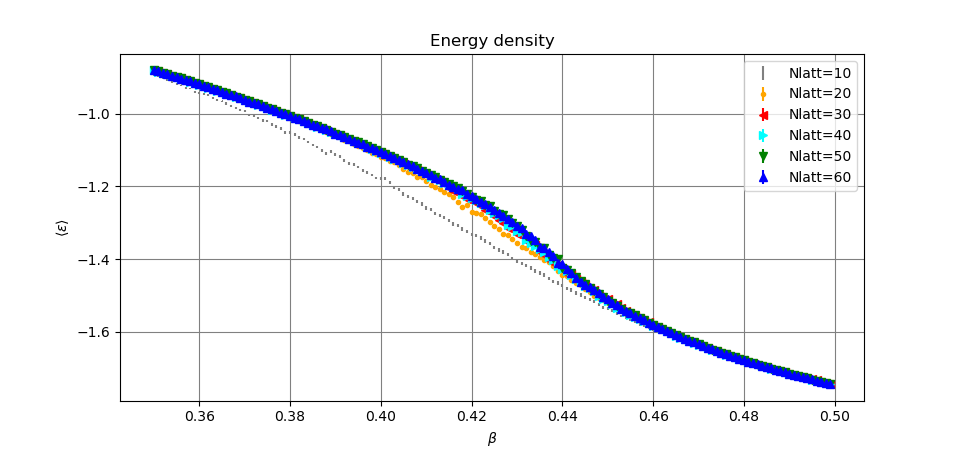
\includegraphics[width=0.95\textwidth]{figures/energy_density.png}
\end{figure}
\begin{figure}
	\centering
	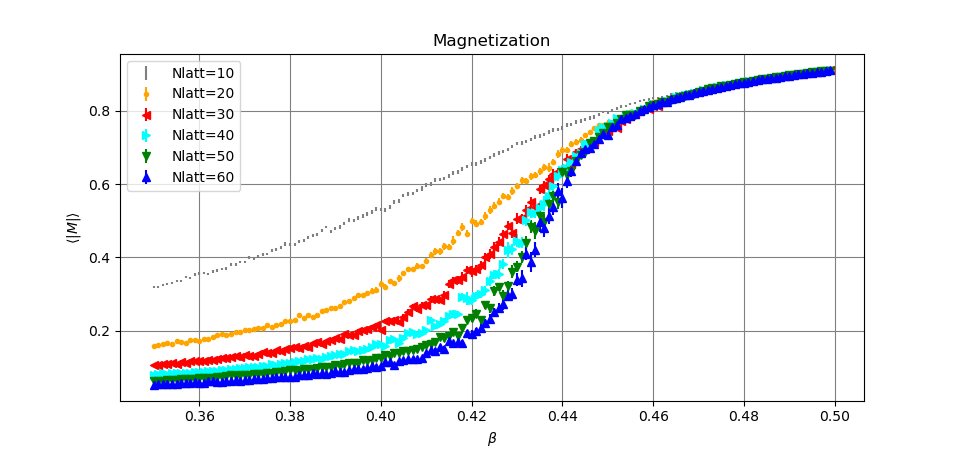
\includegraphics[width=0.95\textwidth]{figures/magnetization_density.png}
\end{figure}
\begin{figure}
	\centering
	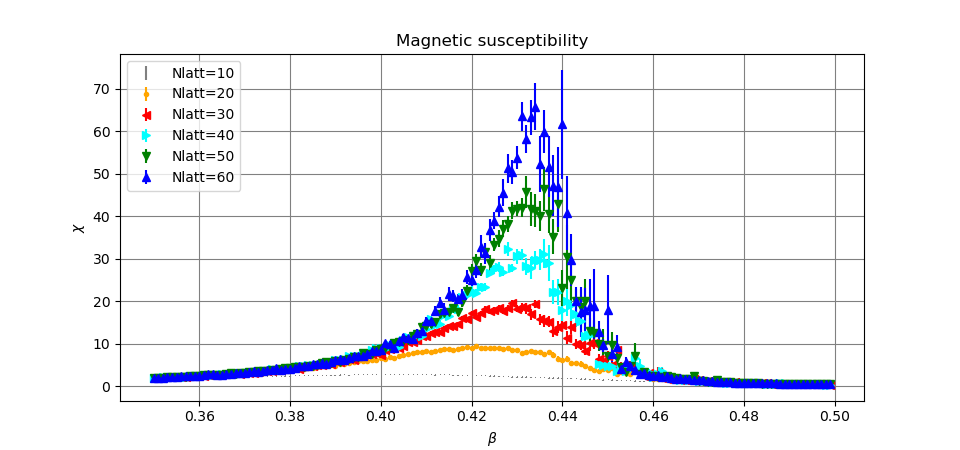
\includegraphics[width=0.95\textwidth]{figures/magnetic_susceptibility.png}
\end{figure}
\begin{figure}
	\centering
	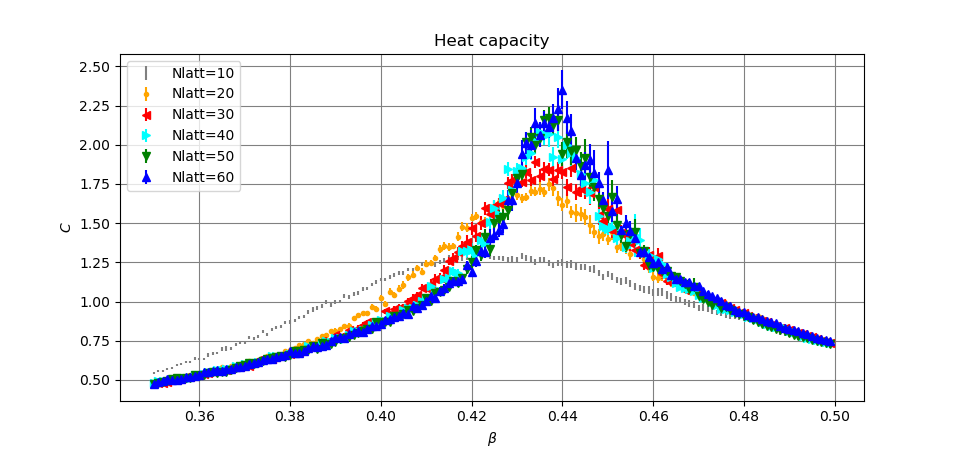
\includegraphics[width=0.95\textwidth]{figures/heat_capacity.png}
\end{figure}
\begin{figure}
	\centering
	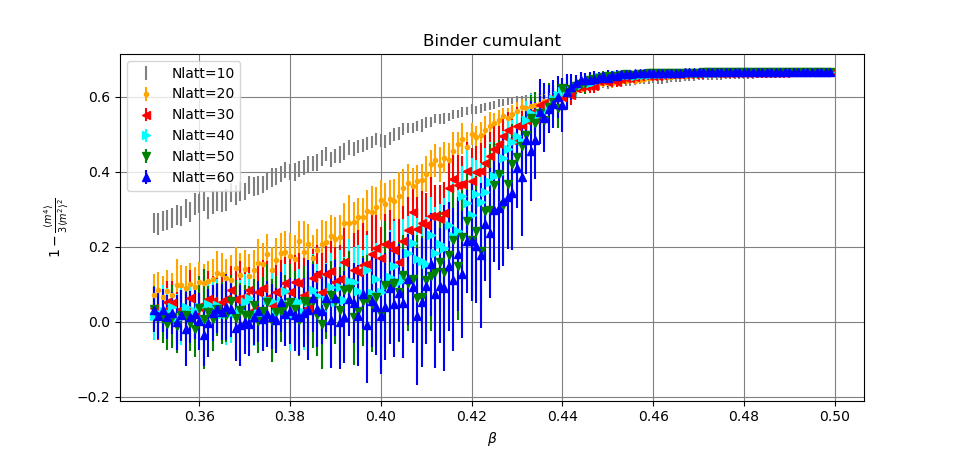
\includegraphics[width=0.95\textwidth]{figures/binder.png}
\end{figure}
From the plots, especially from the susceptibility plot, we can clearly see the limitations of our simulation: the finite size of the system means that we do not observe the continuous phase transition that we would expect in the thermodynamical limit, in fact, in our simulation, the correlation length $\xi$ cannot diverge:
\begin{equation}
\label{limitation}
\xi \leq L
\end{equation}
Which means that the power laws in \eqref{power} can not be satisfied.

\section{Finite Size Scaling}
In order to account for the limitations summarized in \eqref{limitation}, we relied on Finite Size Scaling (FSS). Let us focus our attention on the susceptibility $\chi$, knowing that what follows can be easily transposed onto the other quantities defined in \eqref{power}. In the thermodynamical limit we have:
\begin{equation}
\chi \sim \abs{\xi} ^{\gamma / \nu}
\end{equation}
We know that the quantities that we have measured during our simulation, which we will call $\chi(\beta , \mathtt{Nlatt})$ to make their dependencies explicit, can not diverge but from \eqref{limitation} we can infer that in a neighbourhood of the peak:
\begin{equation}
\chi(\beta , L) = \chi(\xi , L) = L ^{\gamma / \nu} \hat{\varphi}(\xi,L)
\end{equation}
Where $\xi (\beta)$ is the expected correlation length in the thermodynamical limit at temperature $1/\beta$. Furthermore, during a phase transition, $\xi \rightarrow \infty$, so we expect the system to "lose memory" of its own microscopic structure, i.e. the value of $a$, meaning that we can assume that the only relevant length during the transition is the ratio between the two remaining lengths $L$ and $\xi$, so that:
\begin{equation}
\chi(\beta , L) = L ^{\gamma / \nu} \tilde{\varphi}(L/ \xi)= L ^{\gamma / \nu} \tilde{\phi}\left(tL^{1/\nu}\right) = L ^{\gamma / \nu} \varphi\left(\left(\beta - \beta _c\right) L^{1/\nu}\right)
\end{equation}
\begin{equation}
\label{fss_chi}
L ^{-\gamma / \nu}\chi(\beta , L) = \varphi\left(\left(\beta - \beta _c\right) L^{1/\nu}\right)
\end{equation}

\section{Codes}
\label{codes}
All the codes used in the simulation, although a little messy, are available on \href{https://github.com/mccc03/Modulo1}{GitHub} 

\end{document}